\documentclass{article}
\usepackage{amssymb, amsmath}
\usepackage{graphicx}
\usepackage{epstopdf}
\usepackage[left=1cm, right=2cm, top=1.5cm, bottom=1.2cm]{geometry}
\epstopdfsetup{outdir=./}
\begin{document}
  \begin{figure}[hb]
    Figure 1 is my sample figure.\\
    \centering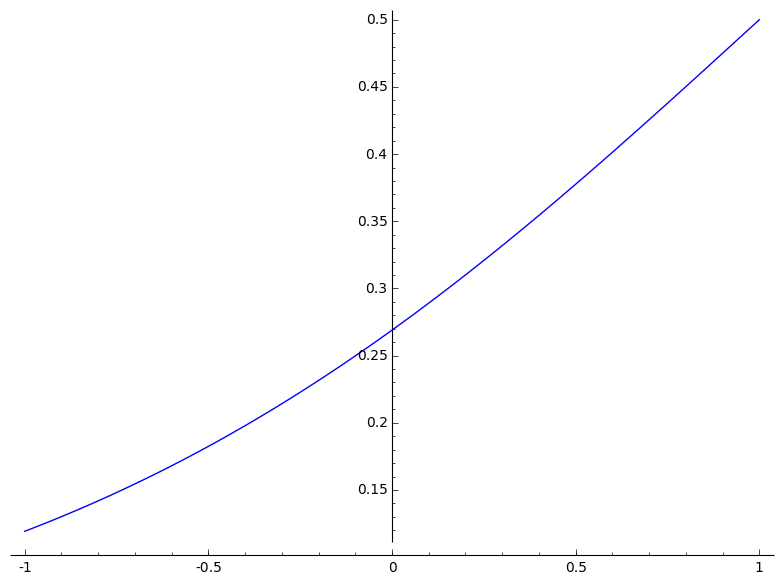
\includegraphics[width=0.3\textwidth]{$PWD/1_1_1.png}
    \caption{A = 1, K = 1, Y = 1}\label{fig:test}
      
    \ \\If you let A bigger, you will find the value is larger in y-axis\\
    \centering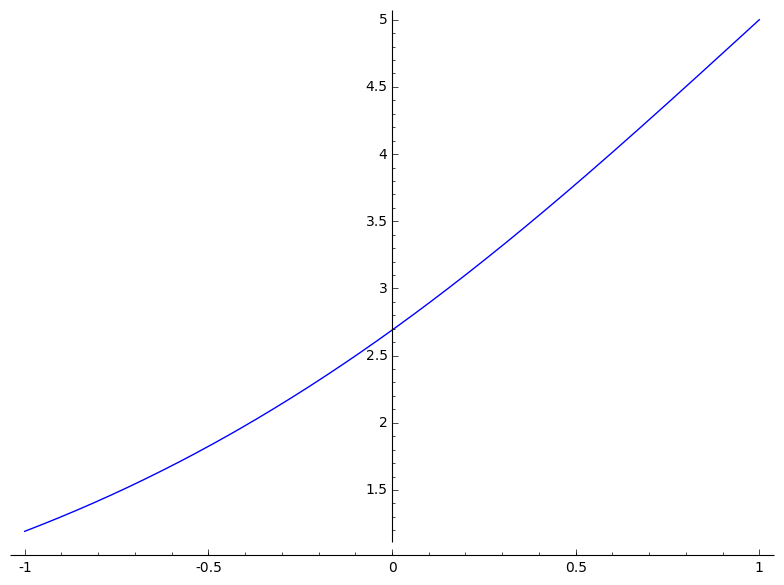
\includegraphics[width=0.3\textwidth]{$PWD/10_1_1.png}
    \caption{A = 10, K = 1, Y = 1}\label{fig:test}
    

    \ \\If you let K bigger, you will find the value of would increase quickly than 1\\
    \centering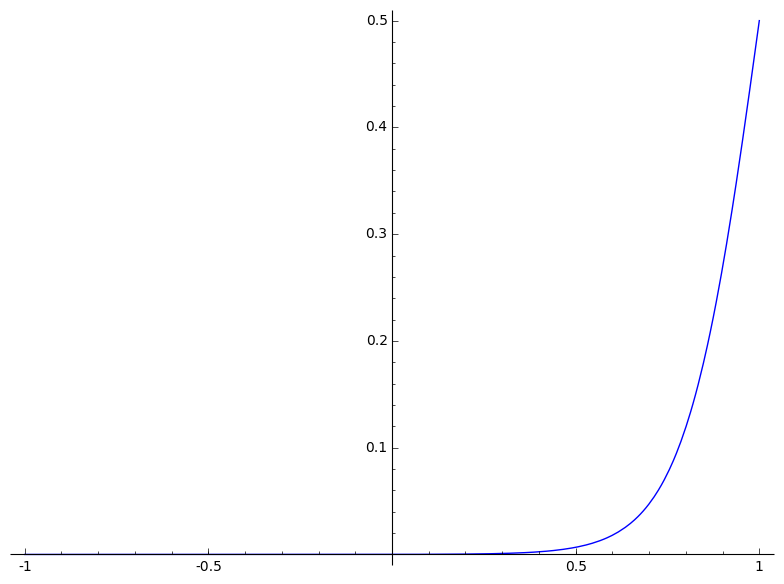
\includegraphics[width=0.3\textwidth]{$PWD/1_10_1.png}
    \caption{A = 1, K = 10, Y = 1}\label{fig:test}
    
    \ \\If you let Y bigger, you will find the shape shift right\\
    \centering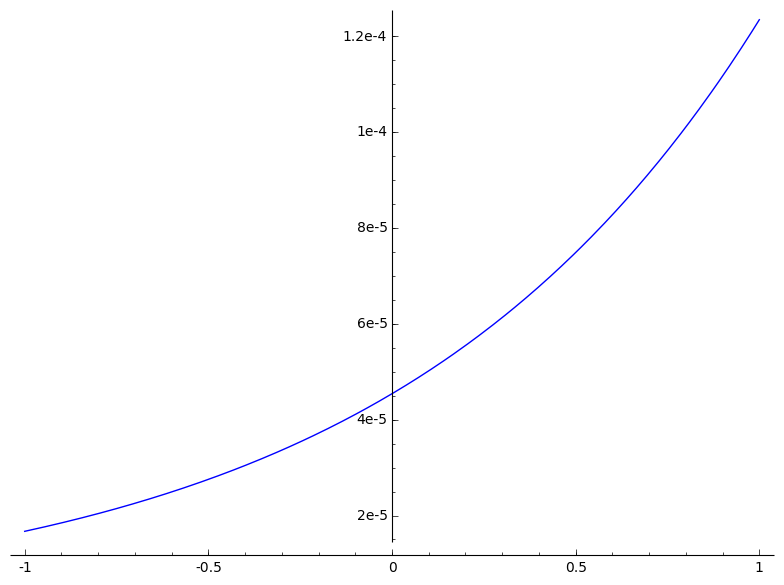
\includegraphics[width=0.3\textwidth]{$PWD/1_1_10.png}
    \caption{A = 1, K = 1, Y = 10}\label{fig:test}
  \end{figure}

\end{document}

